%!TEX root = ../thesis.tex

\chapter[supplementary material: hierarchical vaes know what they don't know]{Supplementary material: Hierarchical VAEs know what they don't know}
\label{app:supplementary-hierarchical}
\ifthenelse{\equal{\skipappendices}{true}}{}{

\section{Datasets} \label{sec_hierarchical:datasets}
\Cref{tab_hierarchical:datasets-overview} lists the datasets used in the paper. We use the predefined train/test splits for the datasets.

For SmallNORB and Omniglot we resize the original grayscale images to $28\times28$ with ordinary bi-linear interpolation.
For each of these datasets, we also create a version where the grayscale is inverted. We do this because, the overall white nature of the images tends to make detecting them as OOD from FashionMNIST artificially easy.
The inversion is done via the simple transformation $\xb_\text{inverted} = 255 - \xb_\text{original}$ since images are encoded as 8 bit unsigned integers.

% Similar to \textcite{serra_input_2020} and \textcite{xiao_likelihood_2020}, we also create a uniform noise dataset ``UniformNoise'' and benchmark our model against this. We dynamically sample each pixel value uniformly as an integer between 0 and 255.

\begin{table}[h!]
    \caption{Overview of the used datasets.}
    \centering
    % \resizebox{0.7\columnwidth}{!}{%
    \begin{tabular}{llr}
        \toprule
        Dataset & Dimensionality & Examples \\
        \midrule
        FashionMNIST \parencite{xiao_fashionmnist_2017} & $28\times28\times1$ & 70,000 \\
        MNIST \parencite{lecun_gradientbased_1998} & $28\times28\times1$ & 70,000 \\
        notMNIST \parencite{bulatov_notmnist_2011} & $28\times28\times1$ & 547,838 \\
        KMNIST \parencite{clanuwat_deep_2018} & $28\times28\times1$ & 70,000 \\
        Omniglot \parencite{lake_humanlevel_2015} & $28\times28\times1$ & 32,460 \\
        SmallNORB \parencite{lecun_learning_2004} & $28\times28\times1$ & 97,200 \\
        % UniformNoise & $28\times28\times1$ & dynamic \\
        \midrule
        CIFAR10 \parencite{krizhevsky_learning_2009} & $32\times32\times3$ & 60,000 \\
        SVHN \parencite{netzer_reading_2011} & $32\times32\times3$ & 99,289 \\
        \bottomrule
    \end{tabular}
    % }
    \label{tab_hierarchical:datasets-overview}
\end{table}


\section{Model details}\label{sec_hierarchical:model-details}
In \cref{tab_hierarchical:hyperparameters} we specify the hyperparameters used when training our models.
We make our source code available at \url{https://github.com/JakobHavtorn/hvae-oodd}.

\subsection{Hierarchical VAE}
Our Hierarchical VAE (HVAE) model uses bottom-up inference and top-down generative paths as specified in the paper.
For grayscale images, the output is parameterized by a Bernoulli distribution while for natural images we use a Discretized Logistic Mixture \parencite{salimans_pixelcnn_2017}.
The latent variables are parameterized by stochastic layers that output the mean and log-variance of a diagonal covariance Gaussian. The prior distribution on the top-most latent is a standard Gaussian.
For grayscale images, the lowest latent space is parameterized by a convolutional neural network and has dimensions $14\times14\times8$ interpreted as (height $\times$ width $\times$ latent dimension). The highest two latent variables are parameterized by dense transformations with $16$ and $8$ units, respectively.
For natural images, the bottom-two latent variables are parameterized by convolutional neural networks and have dimensions $(16\times16)\times128$, $(8\times8)\times64$, respectively for $\zb_1, \zb_2$. The top-most latent, $\zb_3$, is densely connected with dimension $32$.

Each stochastic layer is preceded by a deterministic transformation.
For both grayscale and natural images, each deterministic transformation consists of three residual blocks of the same type used by \textcite{maaloe_biva_2019}. The structure of a residual block is:
\begin{equation}
    \yb = \textsc{conv}\left( \textsc{act} \left( \textsc{conv}_s \left( \textsc{act}(\xb) \right) \right) \right) + \xb \ ,
\end{equation}
where \textsc{conv} refers to a same-padded convolution and \textsc{act} to the activation function. Within a residual block, the first convolution always has stride 1 while the second convolution has stride $s$. In a deterministic transformation, any non-unit stride is performed in the third residual block. For grayscale images, we stride by 2 in the first and second deterministic transformations but not the third. For natural images, we similarly stride by 2 in the first and second deterministic transformations. For grayscale we use 64 channels while we use 256 for natural images.
In both cases, the first deterministic block uses a kernel size of 5 and the latter two a kernel of size 3. We use the ReLU activation function \parencite{fukushima_neocognitron_1980, nair_rectified_2010}.

Since the benefits and drawbacks of using batch normalization \parencite{ioffe_batch_2015} in hierarchical VAEs is still the matter of some debate \parencite{sonderby_ladder_2016, vahdat_nvae_2020, child_very_2021} we choose to use weight normalization \parencite{salimans_weight_2016} as in other work \parencite{maaloe_biva_2019} and initialize the model using the originally proposed data-dependent initialization.
To have the stochastic layers initialize to standard Gaussian distributions (zero mean, unit variance), with this initialization, we select the activation function for the variance as a Softplus,
\begin{equation*}
    \textsc{softplus}(\xb) = \frac{1}{\beta}\log\left(1 + \exp(\beta\xb)\right) \ ,
\end{equation*}
with $\beta = \log(2) \approx 0.693$ to output 1 for $\xb = 0$.

Training of a HVAE model took approximately two days on a single NVIDIA GTX 1080 Ti graphics card.


\subsection{BIVA}
For the BIVA model \parencite{maaloe_biva_2019}, we use a specification that is very similar to that of the HVAE above, and to that of the original paper.
The model has 10 latent variables the lowest 3 of which are spatial and the rest are densely connected in order to have an architecture similar to the HVAE.
The model uses an overall stride of 8, achieved by striding by 2 in the first, fourth and sixth deterministic transformations.
From $\zb_1$ to $\zb_{10}$, the latents have the following dimensions: The lowest three latents are spatial $(16\times16)\times8$, $(16\times16)\times16$ and $(16\times16)\times32$, given as $(\text{height}\times\text{width})\times\text{dim})$, while the rest are dense vectors with dimensions of $42, 40, 38, 36, 34, 32, 30$.

Training of a BIVA model took approximately a week on a single NVIDIA GTX 1080 Ti graphics card.


\begin{table}[t]
    \caption[Selection of most important hyperparameters]{Selection of most important hyperparameters and their setting. Convolutional kernels are square and latent dimensions are given without spatial dimensions which are given in the text. See \cref{sec_hierarchical:model-details} for more details.}
    \centering
    % \resizebox{\columnwidth}{!}{%
    \begin{tabular}{ll}
        \toprule
        Hyperparameter & Setting/Range \\
        \midrule
        \multicolumn{2}{l}{\textbf{All}} \\
        \midrule
        Optimization & Adam \parencite{kingma_adam_2015} \\
        Learning rate & $3e-4$ \\
        Batch size & 128 \\
        Epochs & 2000 \\
        Free bits & $\SI{2}{nats}$ per $\zb_i$ shared across latent dim. \\
        Free bits constant & 200 epochs \\
        Free bits annealed & 200 epochs \\
        Activation & ReLU \\
        \multirow{2}{*}{Initialization} & Data-dependent \\
        & \parencite{salimans_weight_2016} \\
        \midrule
        \multicolumn{2}{l}{\textbf{HVAE}} \\
        Latent dimensionality & 128-64-32 (natural) / 8-16-8 (grey) \\
        Convolution kernel & 5-3-3 \\
        Stride & 2-2-1 \\
        Warmup anneal period & 200 epochs \\
        \midrule
        \multicolumn{2}{l}{\textbf{BIVA}} \\
        \multirow{2}{*}{Latent dimensionality} & 10-8-6 (spatial) \\
        & 42-40-38-36-34-32-30 (dense) \\
        Convolution kernel & 5-3-3-3-3-3-3-3-3-3 \\
        Stride & {2-1-1-2-1-2-1-1-1-1} \\
        \bottomrule
    \end{tabular}
    % }
    \label{tab_hierarchical:hyperparameters}
\end{table}


\section{Analysis of the influence of latent variables on the marginal likelihood} \label{sec_hierarchical:analysis}
In the paper, we argue that the lowest level latent variables, which have the highest dimensionality, contribute the most to the approximate likelihood.
Here, we provide a stringent mathematical argument that generalizes this to the exact marginal likelihood in a model with a deterministic decoder.

\subsection{Model specification}
For an arbitrary hierarchical latent variable model, we have a prior $p(\zb_L)$ and a generative mapping $f: \mathbb{R}^d \rightarrow \mathbb{R}^D$, such that $\xb = f(\zb_L)$ and $D>d$.
Note that we will assume that $f$ is deterministic, such that we are effectively working with $p(\xb|\zb) = \delta_{f(\zb)}(\xb)$.
This is a limiting assumption, but it allows working through the following. For shorthand we will simply write $\zb=\zb_L$.

Let $f$ have a bottleneck architecture, i.e.\
\begin{align}
f(\zb) &= f_1(\ldots f_{L-1}(f_L(\zb))) \ ,
\end{align}
where
\begin{align}
    f_i: \mathbb{R}^{d_{i}} \rightarrow \mathbb{R}^{d_{i-1}}, \qquad i = L, \ldots, 1 \ .
\end{align}
Here we use the notation $d_0=D=\vert\xb\vert$ and $d_L=d=\vert\zb\vert$ and further assume $d_0\geq d_1\geq \ldots \geq d_{L-1} \geq d_L$ which gives the bottleneck.
%$d_1 = d$ and $d_{L+1} = D$ and further assume $d = d_1 \leq d_2 \leq \ldots \leq d_L \leq d_{L+1} = D$ which gives the bottleneck.

Assuming $\xb$ is such that a corresponding latent variable $\zb$ exists, i.e.\ that there exists $\zb$ such that $\xb = f(\zb)$, then we can write the likelihood of $\xb$ through a standard change of variables (similar to flow-based models),
\begin{align}
    p(\xb) &= p(\zb) \prod_{i = 1}^L \left(\sqrt{\det \Jb_i^T \Jb_i}\right)^{-1} \ ,
\end{align}
where $\Jb_i$ is the Jacobian of $f_i$, i.e.
\begin{align}
    \Jb_i &= \frac{\partial f_i}{\partial \zb_i} \in \mathbb{R}^{d_i\times d_{i-1}} \ .
\end{align}
Here we use the notation that $\zb_i$ is the representation at layer $i$.
Note that $\Jb_i^T \Jb_i$ is a $d_{i-1} \times d_{i-1}$ symmetric positive semidefinite matrix (determinant $\geq 0$).

The log-likelihood can be written as
\begin{equation}
    \log p(\xb) = \log p(\zb) - \frac{1}{2} \sum_{i=1}^L \log \det \Jb_i^T\Jb_i \ .
\end{equation}

By construction of determinants, we can generally expect these determinants to grow with the dimensionality of the matrix.
We should expect the determinant of a $d \times d$ matrix to be of the order $\mathcal{O}(\lambda^d)$ for some number $\lambda>0$.
With that in mind, we should generally expect that
\begin{align}
    \det \Jb_{i+1}^T \Jb_{i+1} < \det \Jb_i^T \Jb_i \ ,
\end{align}
due to the bottleneck assumption.
If so, we see that the marginal likelihood $p(\xb)$ will be dominated by $\left(\sqrt{\det \Jb_1^T \Jb_1}\right)^{-1}$, i.e.\ low-level features have a higher influence on the likelihood than more important semantic ones.

\subsection{The Gaussian case}
%
\begin{figure}[t]
    \centering
    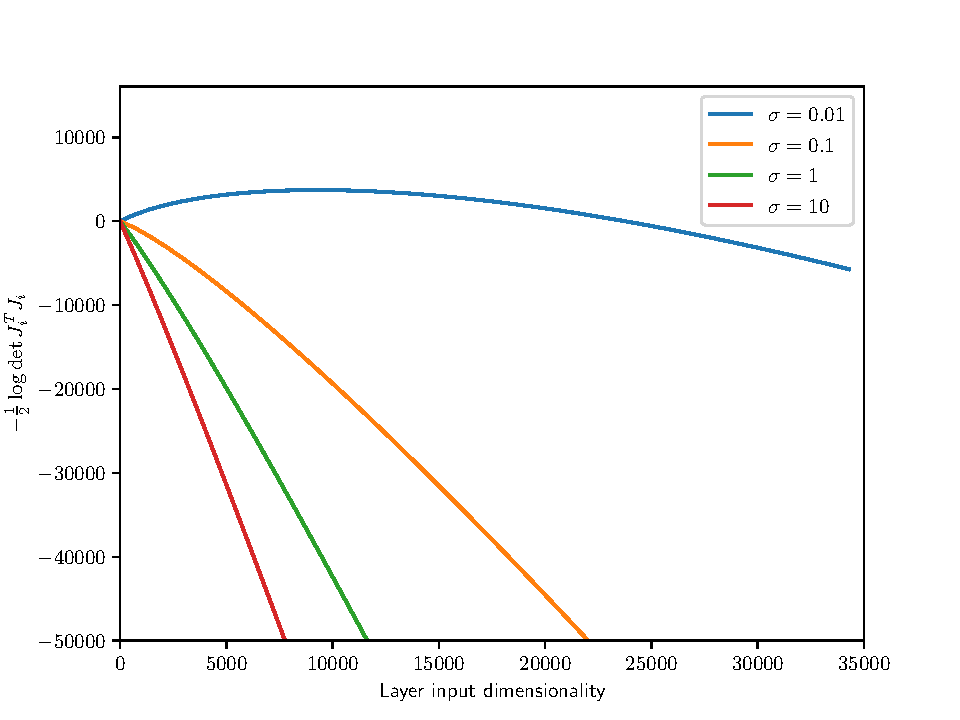
\includegraphics[width=\columnwidth]{paper_hierarchical/logdet2.pdf}
    \caption{The expected inverse volume change for Gaussian Jacobians \eqref{eq_hierarchical:Edet} on a log-scale.}
    \label{fig_hierarchical:Edet}
\end{figure}
The previous remarks can be made more precise if we make distributional assumptions on the Jacobians.
Here we will assume that the Jacobians of each layer follow a Gaussian distribution.
Specifically, we will assume that each entry in $\Jb_i$ is distributed as $\mathcal{N}(0, \sigma^2)$.
The analysis below extends to nonzero means and more general covariance structure, but this comes with a cost of less transparent notation.
In this setting, $\Jb_i^T \Jb_i$ follows a Wishart distribution (in the general setting it would follow a non-central Wishart distribution).
\textcite{muirhead_aspects_2009} tells us that the expected multiplicative contribution to the likelihood of each layer is
\begin{align}
    \mathbb{E}\left[ \left(\sqrt{\det \Jb_i^T \Jb_i}\right)^{-1} \right]
    &= \sigma^{-d_{i-1}}  2^{-\frac{d_{i-1}}{2}} \frac{\Gamma_{d_{i-1}}\left( \frac{1}{2} d_{i} - \frac{1}{2} \right)}{\Gamma_{d_{i-1}}\left( \frac{1}{2} d_{i} \right)} \notag \\
    &= \sigma^{-d_{i-1}}  2^{-\frac{d_{i-1}}{2}} \frac{\Gamma\left( \frac{1}{2} (d_{i} - d_{i-1}) \right)}{\Gamma\left( \frac{1}{2} d_{i} \right)}
    \label{eq_hierarchical:Edet}
\end{align}
where $\Gamma_d$ is the multivariate Gamma function.
Assuming that the increase in layer dimension $d_{i} - d_{i-1}$ is constant, then we see that \eqref{eq_hierarchical:Edet} goes to zero as $d_{i}$ goes to infinity as the $\Gamma$ function grows super-exponentially to infinity.
This super-exponential growth further implies that the first layers dominate the marginal likelihood $p(\xb)$.
This is also visually evident in \cref{fig_hierarchical:Edet}.

\section{Derivation of the \texorpdfstring{$\mathcal{L}^{>k}$}{Lk} bound} \label{sec_hierarchical:derivation_L_geq_k}
In this section we present the derivation of $\mathcal{L}^{>k}$ and show that it is a lower bound on the marginal likelihood.

First, we consider a two-layered VAE with bottom-up inference.
We proceed very similarly to the derivation of the regular ELBO and also use Jensen's inequality.
\begin{align}
\log p(\xb) &= \log \int\int p(\xb|\zb_1)p(\zb_1|\zb_2)p(\zb_2) \text{d}\zb_1\text{d}\zb_2 \\
&\qquad = \log \int\int \frac{q(\zb_2|\xb)}{q(\zb_2|\xb)} p(\xb|\zb_1)p(\zb_1|\zb_2)p(\zb_2) \text{d}\zb_1\text{d}\zb_2 \notag \\
&\qquad = \log \int\int q(\zb_2|\xb) p(\zb_1|\zb_2) \frac{p(\xb|\zb_1)p(\zb_2)}{q(\zb_2|\xb)} \text{d}\zb_1\text{d}\zb_2 \notag \\
%&\ge \mathbb{E}_{p(\zb_1|\zb_2)} \left [ \log q(\zb_2|\xb) \frac{p(\xb|\zb_1)p(\zb_2)}{q(\zb_2|\xb)} \right ] \notag \\
&\ge \mathbb{E}_{p(\zb_1|\zb_2)q(\zb_2|\xb)} \left [ \log \frac{p(\xb|\zb_1)p(\zb_2)}{q(\zb_2|\xb)} \right ] \equiv \mathcal{L}^{> 1} \notag \ .
\end{align}
Here, we have introduced the variational distribution $q(\zb_2|\xb)$ which, naively, is different from any of the available variational distributions $q(\zb_1|\xb)$ and $q(\zb_2|\zb_1)$.
However, it's easy to see that we can simply define $q(\zb_2|\xb)=q(\zb_2|d_1(\xb))$ where $d_1(\xb) = \mathbb{E}\left[q(\zb_1|\xb)\right]$. I.e.\@ we compute the distribution over $\zb_2$ via the mode of $q(\zb_1|\xb)$.
This is possible since we exclusively manipulate the variational proposal distribution without altering the generative model $p(\xb,\zb)$.

In general, the derivation of $\mathcal{L}^{>k}$ for an $L$-layered hierarchical VAE with $\zb=\zb_1,\dots,\zb_L$ is as follows:
\begin{align}
    \log p(\xb) &= \log \int p(\xb|\zb)p(\zb) \text{d}\zb \\
    &\qquad = \log \int \frac{q(\zb_{>k}|\xb)}{q(\zb_{>k}|\xb)} p(\xb|\zb)p(\zb) \text{d}\zb \notag \\
    &\qquad = \log \int q(\zb_{>k}|\xb) p(\zb) \frac{p(\xb|\zb)}{q(\zb_{>k}|\xb)} \text{d}\zb \notag \\
    &\qquad = \log \int q(\zb_{>k}|\xb) p(\zb_{\leq k}|\zb_{>k}) p(\zb_{>k}) \frac{p(\xb|\zb)}{q(\zb_{>k}|\xb)} \text{d}\zb \notag \\
    &\qquad = \log \int q(\zb_{>k}|\xb) p(\zb_{\leq k}|\zb_{>k}) \frac{p(\xb|\zb)p(\zb_{>k})}{q(\zb_{>k}|\xb)} \text{d}\zb \notag \\
    &\qquad \ge \mathbb{E}_{p(\zb_{\leq k}|\zb_{>k})} \left[ \log q(\zb_{>k}|\xb) \frac{p(\xb|\zb)p(\zb_{>k})}{q(\zb_{>k}|\xb)} \right] \notag \\
    &\qquad \ge \mathbb{E}_{p(\zb_{\leq k}|\zb_{>k})q(\zb_{>k}|\xb)} \left[ \log \frac{p(\xb|\zb)p(\zb_{>k})}{q(\zb_{>k}|\xb)} \right] \equiv \mathcal{L}^{>k} \notag \ .
\end{align}
Similar to the $L=2$ case above, we have defined
$$q(\zb_{>k}|\xb) = q(\zb_{>k}|d_k(\xb))$$
with $d_k$ defined recursively as
$$d_k(\xb) = \mathbb{E}\left[q(\zb_k|d_{k-1}(\xb))\right], \qquad d_0(\xb) = \xb\ .$$
That is, we simply consider the inference network below $\zb_{k+1}$ to be a deterministic encoder and forward pass the mode of each preceding variational distribution.

Additionally, we obtain $p(\zb_{\leq k}|\zb_{>k}) p(\zb_{>k})$ by splitting
$$p(\zb)=p(\zb_L)p(\zb_{L-1}|\zb_L)\cdots p(\zb_{1}|\zb_2)$$
at index $k$. Importantly, we then evaluate
$$p(\zb_{>k})=p(\zb_L)p(\zb_{L-1}|\zb_L)\cdots p(\zb_{k+1}|\zb_{k+2})$$
with samples from $q(\zb_{>k}|\xb)$ while
$$p(\zb_{\leq k}|\zb_{>k})=p(\zb_{k}|\zb_{k+1})p(\zb_{k-1}|\zb_{k})\cdots p(\zb_{1}|\zb_{2})$$
is evaluated for $\zb_k$ with $\zb_{k+1} \sim q(\zb_{>k}|\xb)$ and for $\zb_{<k}$ with $\zb_{>k}$ obtained conditionally from itself.

\section{The complementary \texorpdfstring{$\mathcal{L}^{<l}$}{Ll} bound} \label{sec_hierarchical:complementary-bound}
We can generalize the $\mathcal{L}^{>k}$ bound by introducing the flipped version, $\mathcal{L}^{<l}$, which compared to $\mathcal{L}^{>k}$, instead samples the $L-l$ \textit{highest} latent variables in the hierarchy from the prior $\zb_{l},\dots,\zb_L \sim p_\theta(\zb_{\geq l})=p_\theta(\zb_l|\zb_{l+1})\cdots p_\theta(\zb_L)$ and the remaining lower latents from the approximate posterior $\hat{\zb}_{1},\dots,\hat{\zb}_{l-1} \sim q_\phi(\zb_{<l}|\xb)=q_\phi(\zb_{1}|\xb)q_\phi(\zb_{2}|\zb_1)\cdots q_\phi(\zb_{l-1}|\zb_{l-2})$,
\begin{equation}\label{eq_hierarchical:biva-<l}
    \mathcal{L}^{<l} = \mathbb{E}_{p_\theta(\zb_{\geq l}) q_\phi(\zb_{<l}|\xb)} \left[ \log \frac{p_\theta(\xb,\zb)p_\theta(\zb_{<l})}{q_\phi(\zb_{<l}|\xb)} \right].
\end{equation}
Similar to $\mathcal{L}^{>k}$, we recover the regular ELBO for $l=L$. Contrary to $\mathcal{L}^{>k}$, this bound puts as much emphasis on the lowest latent variables as the regular ELBO but keeps track of large deviation from the unconditional prior in the top $L-l$ KL-terms since it is not guided by the approximate posterior for $\zb_{>l}$. We hypothesize that this bound might be useful for OOD detection in cases where the discriminating factor is to be found in low-level statistics rather than high-level features.

Additionally, we can incorporate it in a generalized log likelihood-ratio between $\mathcal{L}^{<l}$ and $\mathcal{L}^{>k}$
\begin{equation}
    LLR^{>k}_{<l} = \mathcal{L}^{<l} - \mathcal{L}^{>k}.
\end{equation}
We hypothesize that this score, or the other possible permutations of it, might be useful for OOD detection but leave further examination to future work.

% While this bound is not expected to improve OOD detection by itself, mainly since the data likelihood $p(\xb|\zb)$ is the same as for the ELBO, we introduce a log likelihood-ratio between $\mathcal{L}^{<l}$ and the regular ELBO, as we did for $\mathcal{L}^{>k}$.
% \begin{equation}
    %     LLR^{<l} = \mathcal{L}^{<l} - \mathcal{L}
    % \end{equation}
    % We hypothesize that this log-likelihood ratio might also be useful for OOD detection based on a more low-level set of semantics learned by the bottom-most latents in the bottom-up hierarchy.
    
    % \section{Generalized log-likelihood ratio $LLR^{>k}_{<l}$}
    % We can further generalize the log-likelhood ratio $LLR^{>k}$ by replacing the ELBO $\mathcal{L}$ with the bound in \eqref{eq_hierarchical:biva-<l} to obtain
    % \begin{equation}
        %     LLR^{>k}_{<l} = \mathcal{L}^{<l} - \mathcal{L}^{>k}.
% \end{equation}


\section{Note on the KL-term of hierarchical VAEs}
In this research we choose model parameterizations relying on bottom-up inference \parencite{burda_importance_2016},
\begin{equation}
    q_\phi(\zb|\xb) = q_\phi(\zb_1|\xb)\textstyle\prod_{i=2}^{L} q_\phi(\zb_i|\zb_{i-1}) \ .
\end{equation}
We do this because bottom-up inference enables the model to learn covariance between the latent variables in the hierarchy.
In the inference model, any latent variable is dependent on the latent variables below it in the hierarchy and, importantly, the top most latent variable is dependent on all other latent variables.

In contrast, a top-down inference model \parencite{sonderby_ladder_2016} has a topmost latent variable $\zb_L$ that is independent of the other latent variables and is directly given by $\xb$.
\begin{equation}
    q_\phi(\zb|\xb) = q_\phi(\zb_L|\xb)\textstyle\prod_{i=L-1}^{1} q_\phi(\zb_{i}|\zb_{i+1}) \ .
\end{equation}
This, in essence, makes $\zb_L$ a mean-field approximation without any covariance structure tying it to the other latent variables, $\text{Cov}(z_{L,i}, z_{k,j})=0$ for $k<L$.
Furthermore, since the approximate posterior (and the prior) typically have diagonal covariance, $\zb_L$ is also mean-field within its own elements, $\text{Cov}(z_{L,i}, z_{L,j})=0$ for $i\ne j$.

We hypothesize that the covariance of latent variables towards the top of the hierarchy with other latent variables is important for learning semantic representations.
However, top-down inference models are easier to optimize as has recently been demonstrated \parencite{sonderby_ladder_2016, vahdat_nvae_2020, child_very_2021}.

In the following, we inspect the differences between the ELBO used for bottom-up inference and the ELBO used for top-down inference and show that it is not generally possible to decompose the total KL-divergence into separate KL-divergences per latent variable.
Specifically, for top-down inference it is possible to obtain KL-divergence at the top-most latent variable and an expectation of a KL-divergence for the other latent variables.
For bottom-up inference, the resulting terms are no longer KL-divergences except at the top-most latent variable.

We ask the question whether models relying on top-down inference are impeded in their use for semantic OOD detection, or whether they still learn to assign a more semantic representation in the top-most variables simply due to the flexibility of the deterministic neural network layers.
This remains an open research question.


\subsection{Bottom-up inference}
% The ELBO for the bottom-up VAE is given by:
% \begin{align}
    %     \log p(\xb) &\ge \mathbb{E}_{q(\zb_1, \zb_2|\xb)} \left[ \log \left(p(\xb|\zb_1) p(\zb_1|\zb_2) p(\zb_2) \right) \notag \\
    %     &\qquad - \log \left( q(\zb_1|\xb) q(\zb_2|\zb_1)\right) \right]\ .
    % \end{align}
    By splitting up the expectation, we can write the ELBO of a two-layer bottom-up hierarchical VAE as
    \begin{align}
        \log p(\xb) &\ge \mathbb{E}_{q(\zb_1, \zb_2|\xb)} \left[ \log p(\xb|\zb_1) \right] \\
    &\qquad + \mathbb{E}_{q(\zb_1,\zb_2|\xb)} \left[ \log p(\zb_1|\zb_2) - \log q(\zb_1|\xb) \right] \notag \\
    &\qquad + \mathbb{E}_{q(\zb_1,\zb_2|\xb)} \left[ \log p(\zb_2) - \log q(\zb_2|\zb_1) \right] \notag \ .
\end{align}
We can write out the expectations in order to derive the KL-divergence terms of the bottom-up ELBO:
\begin{align}
    \log p(\xb) &\ge \int \int \log p(\xb|\zb_1) \text{d}\zb_2\zb_1 \label{eq_hierarchical:2 layer VAE bottom up ELBO integrals} \\
    &\qquad + \int q(\zb_1|\xb) \int q(\zb_2|\zb_1) \log \frac{p(\zb_1|\zb_2)}{q(\zb_1|\xb)} \text{d}\zb_2\zb_1 \notag \\ 
    &\qquad + \int q(\zb_1|\xb) \int q(\zb_2|\zb_1) \log \frac{p(\zb_2)}{q(\zb_2|\zb_1)} \text{d}\zb_2\zb_1 \notag  \ .
\end{align}
From the above, we can see that since the decomposition is in a reverse order, we cannot derive the KL-divergence for the second term. This will hold in general for $L$-layered models for any latent variables  $\zb_1,...,\zb_{L-1}$:
\begin{align}
    \log p(\xb) &\ge \mathbb{E}_{q(\zb_1, \zb_2|\xb)} \left[ \log p(\xb|\zb_1) \right] \\
    &\qquad + \mathbb{E}_{q(\zb_1|\xb)}\left[ \mathbb{E}_{q(\zb_2|\zb_1)}\left[\log \frac{p(\zb_1|\zb_2)}{q(\zb_1|\xb)}\right]\right] \notag \\
    &\qquad + \mathbb{E}_{q(\zb_1|\xb)}\left[-D_\text{KL}[q(\zb_2|\zb_1)\parallel p(\zb_2)]\right] \notag \ .
\end{align}


\subsection{Top-down inference}
% The ELBO for the top-down VAE is given by:
% \begin{align}
    %     \log p(\xb) \ge \mathbb{E}_{q(\zb_1, \zb_2|\xb)} \left[ \log \left(p(\xb|\zb_1) p(\zb_1|\zb_2) p(\zb_2) \right)- \log \left( q(\zb_2|\xb) q(\zb_1|\zb_2)\right) \right]\ .
    % \end{align}
    % By splitting up the expectation we can easily rewrite this ELBO:
    By splitting up the expectation, we can write the ELBO of a two-layer top-down hierarchical VAE as
    \begin{align}
        \log p(\xb) &\ge \mathbb{E}_{q(\zb_1, \zb_2|\xb)} \left[ \log p(\xb|\zb_1) \right] \\ 
        &\qquad + \mathbb{E}_{q(\zb_1,\zb_2|\xb)} \left[ \log p(\zb_2|\xb) - \log q(\zb_2|\xb) \right] \notag \\
        &\qquad + \mathbb{E}_{q(\zb_1,\zb_2|\xb)} \left[ \log p(\zb_1|\zb_2) - \log q(\zb_1|\zb_2) \right] \notag \ .
    \end{align}
    We can write out the expectations in order to derive the KL-divergence terms:
    \begin{align}
        \log p(\xb) &\ge \int \int \log p(\xb|\zb_1) d\zb_1\zb_2 \\
        &\qquad + \int q(\zb_2|\xb) \log \frac{p(\zb_2|\xb)}{q(\zb_2|\xb)} d\zb_2 \notag \\ 
        &\qquad + \int q(\zb_2|\xb) \int q(\zb_1|\zb_2) \log \frac{p(\zb_1|\zb_2)}{q(\zb_1|\zb_2)} d\zb_1\zb_2 \notag \ .
    \end{align}
    The KL-divergence terms can now easily be computed by:
    \begin{align}
        \log p(\xb) &\ge \mathbb{E}_{q(\zb_1, \zb_2|\xb)} \left[ \log p(\xb|\zb_1) \right] \\
    &\qquad - D_\text{KL}[q(\zb_2|\xb)\parallel p(\zb_2)] \notag \\ 
    &\qquad - \mathbb{E}_{q(\zb_2|\xb)}\left[D_\text{KL}[q(\zb_1|\zb_2)\parallel p(\zb_1|\zb_2)\right] \notag \ .
\end{align}
Note that the KL-divergence in the second layer is not exact since it is dependent on the sample-noise from the layer below. An exact solution can only be derived if the latent variables $\mathbf{z}$ are all conditionally independent. However, this comes at the cost of not learning a covariance structure.


\section{Additional results} \label{sec_hierarchical:additional-results}
We provide additional results for a model trained on FashionMNIST in \cref{tab_hierarchical:additional-results-fashionmnist}, a model trained on MNIST in \cref{tab_hierarchical:additional-results-mnist}, a model trained on CIFAR10 in \cref{tab_hierarchical:additional-results-cifar} and a model trained on SVHN in \cref{tab_hierarchical:additional-results-svhn}.

We note that while the likelihood is highly unreliable across the datasets, the proposed log likelihood-ratio score is consistent and always allows correct OOD detection with high AUROC$\uparrow$.

\begin{table}[t]
    \caption[Additional results for the HVAE model trained on SVHN]{Additional results for the HVAE model trained on SVHN. All results computed with 1000 importance samples.}
    \centering
    % \resizebox{\columnwidth}{!}{%
    \begin{tabular}{llrrr}
        \toprule
        OOD dataset & Metric & AUROC$\uparrow$ & AUPRC$\uparrow$ & FPR80$\downarrow$ \\
        \midrule
        \multicolumn{5}{c}{\textbf{Trained on SVHN}} \\
        \midrule
        CIFAR10            &  $\mathcal{L}^{>0}$         &  $0.992$  &  $0.993$  &  $0.004$  \\
        CIFAR10            &  $\mathcal{L}^{>1}$         &  $0.988$  &  $0.990$  &  $0.002$  \\
        CIFAR10            &  $\mathcal{L}^{>2}$         &  $0.746$  &  $0.756$  &  $0.468$  \\
        CIFAR10            &  $LLR^{>1}$       &  $0.939$  &  $0.950$  &  $0.052$  \\
        % \midrule
        % UniformNoise       &  $\mathcal{L}^{>0}$         &  $1.000$  &  $1.000$  &  $0.000$  \\
        % UniformNoise       &  $\mathcal{L}^{>1}$         &  $1.000$  &  $1.000$  &  $0.000$  \\
        % UniformNoise       &  $\mathcal{L}^{>2}$         &  $0.965$  &  $0.957$  &  $0.055$  \\
        % UniformNoise       &  $LLR^{>1}$       &  $0.984$  &  $0.992$  &  $0.000$  \\
        \midrule
        SVHN               &  $\mathcal{L}^{>0}$         &  $0.599$  &  $0.587$  &  $0.702$  \\
        SVHN               &  $\mathcal{L}^{>1}$         &  $0.555$  &  $0.543$  &  $0.755$  \\
        SVHN               &  $\mathcal{L}^{>2}$         &  $0.403$  &  $0.431$  &  $0.869$  \\
        SVHN               &  $LLR^{>1}$       &  $0.489$  &  $0.484$  &  $0.799$  \\
        \bottomrule
    \end{tabular}
    % }
    \label{tab_hierarchical:additional-results-svhn}
\end{table}
% Results of SVHN model. (d64aa83013304864b974a3fca31e44f1)

\begin{table}[t]
    \caption[Additional results for the HVAE model trained on CIFAR10]{Additional results for the HVAE model trained on CIFAR10. All results computed with 1000 importance samples.}
    \centering
    % \resizebox{\columnwidth}{!}{%
    \begin{tabular}{llrrr}
        \toprule
        OOD dataset & Metric & AUROC$\uparrow$ & AUPRC$\uparrow$ & FPR80$\downarrow$ \\
        \midrule
        \multicolumn{5}{c}{\textbf{Trained on CIFAR10}} \\
        \midrule
        SVHN          &  $\mathcal{L}^{>0}$    &  0.083  &  0.318  &  0.974  \\
        SVHN          &  $\mathcal{L}^{>1}$    &  0.097  &  0.320  &  0.972  \\
        SVHN          &  $\mathcal{L}^{>2}$    &  0.693  &  0.725  &  0.599  \\
        SVHN          &  $LLR^{>2}$  &  0.811  &  0.837  &  0.394  \\
        % \midrule
        % UniformNoise  &  $\mathcal{L}^{>0}$    &  1.000  &  1.000  &  0.000  \\
% UniformNoise  &  $\mathcal{L}^{>1}$    &  0.987  &  0.984  &  0.025  \\
% UniformNoise  &  $\mathcal{L}^{>2}$    &  0.031  &  0.313  &  0.971  \\
% UniformNoise  &  $LLR^{>1}$  &  0.206  &  0.436  &  0.999  \\
\midrule
CIFAR10       &  $\mathcal{L}^{>0}$    &  0.485  &  0.488  &  0.817  \\
CIFAR10       &  $\mathcal{L}^{>1}$    &  0.467  &  0.476  &  0.822  \\
CIFAR10       &  $\mathcal{L}^{>2}$    &  0.411  &  0.433  &  0.869  \\
CIFAR10       &  $LLR^{>1}$  &  0.469  &  0.479  &  0.835  \\
         \bottomrule
    \end{tabular}
    % }
    \label{tab_hierarchical:additional-results-cifar}
\end{table}
% CIFAR10 model: 94f41e80fde444478403496071289a75


\begin{table}[t]
    \caption[Additional results for the HVAE model trained on FashionMNIST]{Additional results for the HVAE model trained on FashionMNIST. All results computed with 1000 importance samples.}
    \centering
    % \resizebox{\columnwidth}{!}{%
    \begin{tabular}{llrrr}
        \toprule
         OOD dataset & Metric & AUROC$\uparrow$ & AUPRC$\uparrow$ & FPR80$\downarrow$ \\
         \midrule
         \multicolumn{5}{c}{\textbf{Trained on FashionMNIST}} \\
         \midrule
MNIST                    & $\mathcal{L}^{>0}$     &  0.268  &  0.363  &  0.882 \\
MNIST                    & $\mathcal{L}^{>1}$     &  0.593  &  0.591  &  0.658 \\
MNIST                    & $\mathcal{L}^{>2}$     &  0.712  &  0.750  &  0.548 \\
MNIST                    & $LLR^{>1}$             &  0.986  &  0.987  &  0.011 \\
\midrule
notMNIST                 &  $\mathcal{L}^{>0}$    &  0.916  &  0.932  &  0.116 \\
notMNIST                 &  $\mathcal{L}^{>1}$    &  0.983  &  0.986  &  0.000 \\
notMNIST                 &  $\mathcal{L}^{>2}$    &  0.997  &  0.997  &  0.000 \\
notMNIST                 &  $LLR^{>1}$            &  0.998  &  0.998  &  0.000 \\
\midrule
KMNIST                   &  $\mathcal{L}^{>0}$    &  0.690  &  0.694  &  0.554 \\
KMNIST                   &  $\mathcal{L}^{>1}$    &  0.835  &  0.863  &  0.359 \\
KMNIST                   &  $\mathcal{L}^{>2}$    &  0.844  &  0.875  &  0.339 \\
KMNIST                   &  $LLR^{>1}$            &  0.974  &  0.977  &  0.017 \\
\midrule
Omniglot28x28            &  $\mathcal{L}^{>0}$    &  0.898  &  0.837  &  0.166 \\
Omniglot28x28            &  $\mathcal{L}^{>1}$    &  0.991  &  0.989  &  0.011 \\
Omniglot28x28            &  $\mathcal{L}^{>2}$    &  1.000  &  1.000  &  0.000 \\
Omniglot28x28            &  $LLR^{>2}$            &  1.000  &  1.000  &  0.000 \\
\midrule
Omniglot28x28Inverted    &  $\mathcal{L}^{>0}$    &  0.261  &  0.361  &  0.879 \\
Omniglot28x28Inverted    &  $\mathcal{L}^{>1}$    &  0.450  &  0.431  &  0.709 \\
Omniglot28x28Inverted    &  $\mathcal{L}^{>2}$    &  0.557  &  0.574  &  0.678 \\
Omniglot28x28Inverted    &  $LLR^{>1}$            &  0.954  &  0.954  &  0.050 \\
\midrule
SmallNORB28x28           &  $\mathcal{L}^{>0}$    &  0.982  &  0.984  &  0.000 \\
SmallNORB28x28           &  $\mathcal{L}^{>1}$    &  0.998  &  0.998  &  0.000 \\
SmallNORB28x28           &  $\mathcal{L}^{>2}$    &  1.000  &  1.000  &  0.000 \\
SmallNORB28x28           &  $LLR^{>2}$            &  0.999  &  0.999  &  0.002 \\
\midrule
SmallNORB28x28Inverted   &  $\mathcal{L}^{>0}$    &  0.965  &  0.971  &  0.000 \\
SmallNORB28x28Inverted   &  $\mathcal{L}^{>1}$    &  0.997  &  0.992  &  0.000 \\
SmallNORB28x28Inverted   &  $\mathcal{L}^{>2}$    &  0.981  &  0.985  &  0.000 \\
SmallNORB28x28Inverted   &  $LLR^{>2}$            &  0.941  &  0.946  &  0.069 \\
% \midrule
% UniformNoise             &  $\mathcal{L}^{>0}$    &  1.000  &  1.000  &  0.000 \\
% UniformNoise             &  $\mathcal{L}^{>1}$    &  1.000  &  1.000  &  0.000 \\
% UniformNoise             &  $\mathcal{L}^{>2}$    &  1.000  &  1.000  &  0.000 \\
% UniformNoise             &  $LLR^{>2}$            &  0.997  &  0.996  &  0.004 \\
\midrule
FashionMNIST             &  $\mathcal{L}^{>0}$    &  0.476  &  0.484  &  0.816 \\
FashionMNIST             &  $\mathcal{L}^{>1}$    &  0.475  &  0.482  &  0.817 \\
FashionMNIST             &  $\mathcal{L}^{>2}$    &  0.475  &  0.484  &  0.823 \\
FashionMNIST             &  $LLR^{>1}$            &  0.488  &  0.496  &  0.811 \\
         \bottomrule
    \end{tabular}
    % }
    \label{tab_hierarchical:additional-results-fashionmnist}
\end{table}
% FMNIST model: d65f60927f174ab786a817024a0a4d75.  (alt 0e34596bfe6a4e60a5c0d2bf9440c70d)

\begin{table}[t]
    \caption[Additional results for the HVAE model trained on MNIST]{Additional results for the HVAE model trained on MNIST. All results computed with 1000 importance samples.}
    \centering
    % \resizebox{\columnwidth}{!}{%
    \begin{tabular}{llrrr}
        \toprule
         OOD dataset & Metric & AUROC$\uparrow$ & AUPRC$\uparrow$ & FPR80$\downarrow$ \\
         \midrule
         \multicolumn{5}{c}{\textbf{Trained on MNIST}} \\
         \midrule
FashionMNIST                     &  $\mathcal{L}^{>0}$  &  $1.000$  &  $1.000$  &  $0.000$ \\
FashionMNIST                     &  $\mathcal{L}^{>1}$  &  $1.000$  &  $1.000$  &  $0.000$ \\
FashionMNIST                     &  $\mathcal{L}^{>2}$  &  $0.981$  &  $0.983$  &  $0.003$ \\
FashionMNIST                   &  $LLR^{>1}$  &  $0.999$  &  $0.999$  &  $0.000$ \\
\midrule
notMNIST                         &  $\mathcal{L}^{>0}$  &  $1.000$  &  $1.000$  &  $0.000$ \\
notMNIST                         &  $\mathcal{L}^{>1}$  &  $1.000$  &  $1.000$  &  $0.000$ \\
notMNIST                         &  $\mathcal{L}^{>2}$  &  $1.000$  &  $1.000$  &  $0.000$ \\
notMNIST                       &  $LLR^{>1}$  &  $1.000$  &  $0.999$  &  $0.000$ \\
\midrule
KMNIST                           &  $\mathcal{L}^{>0}$  &  $1.000$  &  $1.000$  &  $0.000$ \\
KMNIST                           &  $\mathcal{L}^{>1}$  &  $1.000$  &  $1.000$  &  $0.000$ \\
KMNIST                           &  $\mathcal{L}^{>2}$  &  $0.987$  &  $0.987$  &  $0.011$ \\
KMNIST                         &  $LLR^{>1}$  &  $0.999$  &  $0.999$  &  $0.000$ \\
\midrule
Omniglot28x28                    &  $\mathcal{L}^{>0}$  &  $1.000$  &  $1.000$  &  $0.000$ \\
Omniglot28x28                    &  $\mathcal{L}^{>1}$  &  $1.000$  &  $1.000$  &  $0.000$ \\
Omniglot28x28                    &  $\mathcal{L}^{>2}$  &  $1.000$  &  $1.000$  &  $0.000$ \\
Omniglot28x28                  &  $LLR^{>1}$  &  $1.000$  &  $1.000$  &  $0.000$ \\
\midrule
Omniglot28x28Inverted            &  $\mathcal{L}^{>0}$  &  $0.862$  &  $0.902$  &  $0.205$ \\
Omniglot28x28Inverted            &  $\mathcal{L}^{>1}$  &  $0.923$  &  $0.943$  &  $0.056$ \\
Omniglot28x28Inverted            &  $\mathcal{L}^{>2}$  &  $0.749$  &  $0.691$  &  $0.411$ \\
Omniglot28x28Inverted          &  $LLR^{>1}$  &  $0.944$  &  $0.953$  &  $0.057$ \\
\midrule
SmallNORB28x28                   &  $\mathcal{L}^{>0}$  &  $1.000$  &  $1.000$  &  $0.000$ \\
SmallNORB28x28                   &  $\mathcal{L}^{>1}$  &  $1.000$  &  $1.000$  &  $0.000$ \\
SmallNORB28x28                   &  $\mathcal{L}^{>2}$  &  $1.000$  &  $1.000$  &  $0.000$ \\
SmallNORB28x28                 &  $LLR^{>1}$  &  $1.000$  &  $1.000$  &  $0.000$ \\
\midrule
SmallNORB28x28Inverted           &  $\mathcal{L}^{>0}$  &  $1.000$  &  $1.000$  &  $0.000$ \\
SmallNORB28x28Inverted           &  $\mathcal{L}^{>1}$  &  $1.000$  &  $1.000$  &  $0.000$ \\
SmallNORB28x28Inverted           &  $\mathcal{L}^{>2}$  &  $0.977$  &  $0.980$  &  $0.001$ \\
SmallNORB28x28Inverted         &  $LLR^{>1}$  &  $0.985$  &  $0.987$  &  $0.000$ \\
% \midrule
% UniformNoise                     &  $\mathcal{L}^{>0}$  &  $1.000$  &  $1.000$  &  $0.000$ \\
% UniformNoise                     &  $\mathcal{L}^{>1}$  &  $1.000$  &  $1.000$  &  $0.000$ \\
% UniformNoise                     &  $\mathcal{L}^{>2}$  &  $1.000$  &  $1.000$  &  $0.000$ \\
% UniformNoise                   &  $LLR^{>1}$  &  $1.000$  &  $1.000$  &  $0.000$ \\
\midrule
MNIST                            &  $\mathcal{L}^{>0}$  &  $0.488$  &  $0.486$  &  $0.807$ \\
MNIST                            &  $\mathcal{L}^{>1}$  &  $0.469$  &  $0.469$  &  $0.816$ \\
MNIST                            &  $\mathcal{L}^{>2}$  &  $0.514$  &  $0.505$  &  $0.791$ \\
MNIST                          &  $LLR^{>2}$  &  $0.515$  &  $0.507$  &  $0.792$ \\
         \bottomrule
    \end{tabular}
    % }
    \label{tab_hierarchical:additional-results-mnist}
\end{table}
% Results of MNIST model. (57bed090cf4a4e44b896b4c2cce55500)
}
